% I would rather have a bit of space between paragraphs
\setlength{\parskip}{0.5\baselineskip}

% I would like to include the abstract at the top
\begin{quote}
\small
\articleABSTRACT
\end{quote}


\section{Introduction}

\citet{lamichhane2003} described a Bayesian statistical method for
estimating the number and identity of essential genes in a genome from
data that indicates viable mutants. The genome of \emph{Mycobacterium
tuberculosis\/} was mutagenized with a transposon that inserted at
known sites, and a library of viable mutants was characterized. If a
mutant with insertion that disrupted a particular gene was viable,
that gene was indicated to be non-essential. Essential genes are those
for which no disruptive mutation could be viable.

The analysis method, described in further detail in
\citet{blades2002}, sought to estimate the overall proportion of
essential genes, and the probability that a gene was essential. We
assumed a uniform prior distribution on the number of essential genes,
and that genes were equally likely to be essential, and used Markov
chain Monte Carlo (MCMC) to derive the posterior probabilities of genes being
essential.

As part of the ReScience Ten Years Reproducibility Challenge, I sought
to reproduce the analyses in the paper, which I conducted in 2002
while in the Department of Biostatistics at
Johns Hopkins University. The bulk of the data and code were quickly
identified. (I keep collaborative projects in a directory
{\tt {\textasciitilde}/Projects} and save old projects in compressed form in
{\tt {\textasciitilde}/Projects/Tar}, and I immediately found
the file {\tt Gyanu.tgz}. Gyanu Lamichhane was first author on the
paper.) However, there were a number of challenges in reconstructing
the analysis steps, and the code used to conduct the computer
simulations underlying Figure~3 from \citet{lamichhane2003} appears
lost; I found only the results and the code to generate the figure.

The method was implemented in a combination of R \citep{R} and C
\citep{C} and assembled as an R package, R/negenes \citep{negenes},
which is available on both
\href{https://github.com/kbroman/negenes}{GitHub} and the
\href{https://cran.r-project.org/package=negenes}{Comprehensive R
  Archive Network (CRAN)}. The software used for the analyses in the
paper are a set of R scripts, along with one Perl script
\citep{Perl} that extracted transposon insertion sites from the \emph{M.\
tuberculosis\/} genome.

\section{Challenges}

The first challenge in reproducing the analyses
in \citet{lamichhane2003} was to identify exactly what analyses needed
to be reproduced. The project directory did not contain any
documentation, and the file organization (Figure~\ref{fig:files}) was
quirky and contained a number of ancillary analyses that did not end
up in the paper. And so I had to resort to actually reading the
original article.



\begin{figure}
\definecolor{offwhite}{RGB}{255,250,240}
\lstset{language=bash,
        basicstyle=\ttfamily\scriptsize,
        frame=single,
        commentstyle=,
        backgroundcolor=\color{offwhite},
        showspaces=false,
        showstringspaces=false
        }

\begin{lstlisting}
class_problems.txt        findTA.pl*        Randomness/
Converge/                 mindGaps.pl*      Rawdata/
crucial_doubleTA.txt      Nov02/            Sept02/
Data/                     Operons/          Sims/
doubleta_hit.txt          R/                TroubleShootingSubClasses.txt
exploreSeq.pl*
\end{lstlisting}

\caption{Project directory for the work\label{fig:files}}
\end{figure}



There was some system behind the organization of the project files,
but it would have benefited from a {\tt ReadMe} file that
explained the structure. The
subdirectories {\tt Converge}, {\tt Operons}, {\tt Randomness},
and {\tt Sims} contain the ancillary analyses that did not end up in the
paper. {\tt Rawdata} contains the primary data files, {\tt Data}
contains derived data files, and {\tt R} contains analysis scripts.

But actually {\tt Rawdata}, {\tt Data}, and {\tt R} contain files
for an initial analysis of the data performed in July, 2002. The subdirectory
{\tt Sept02} contains copies of those data and scripts
for a revised analysis performed in September, 2002; many of the files
are identical, but additional data had been added.
Similarly, {\tt Nov02} contains further copies of the data and
scripts for a further revised analysis performed in November, 2002.

The bulk of the results in the paper are those from {\tt Nov02}.
Table~2 from \citet{lamichhane2003} includes results from {\tt Sept02}
as well as {\tt Nov02}. This was the primary challenge in reproducing
the analyses: identifying which versions of the analysis
scripts were used.

There were a number of further challenges in reproducing the results.
The code to produce Figure~1b from \citet{lamichhane2003} (see
Figure~\ref{fig:fig1b}, below) was not
present in the project directory, but rather was found in a separate
directory, with files for a talk that I gave on the work.

Further, the key analyses involved Markov chain Monte Carlo (MCMC),
but I had not saved the seeds for the random number generator, and so
I am not able to reproduce the results exactly. Also, I did not save
the key intermediate results to files, and I did not indicate which
objects were produced by which scripts. Rather, I left objects in the
R environment (saved in a {\tt .RData} file and re-loaded when R was
invoked) and used them as needed without explaining where they had
come from. Nevertheless, the analysis scripts were reasonably well
named ({\tt prepareData.R}, {\tt analysis.R},
and {\tt figs4paper.R}), and so the order of the analysis could be
reconstructed without much difficulty.

\section{Code modifications}

The original analysis was performed with R version 1.5.1 (2002-06-17);
the reproduction used R version 3.6.2 (2019-12-12). The analysis
scripts could be run with only one small modification. The output of
the R function {\tt table()}, which counts the values in a
categorical variable, is now an object of class {\tt table}, where as
previously it had been a numeric array, and so
I needed to insert a couple of {\tt as.numeric()} calls to avoid
errors.

I also needed to make small changes regarding cutoffs controlling which results
were shown in two key tables. Because I had not saved the seed for
the random number generator, I was not able to reproduce the MCMC
results exactly, and small differences in the estimated posterior
probabilities meant that I needed to change cutoffs from 0.749 to
0.745 in order to display the same set of genes and gene families.




\section{The R/negenes package}

The key software implementing the methods of \citet{lamichhane2003}
is in the R package, R/negenes \citep{negenes}, available on the
\href{https://cran.r-project.org/package=negenes}{Comprehensive R
Archive Network (CRAN)}. The earliest version on CRAN is 0.98-3, dated
2002-08-10 and posted to CRAN on 2003-06-21. This is the version that
was used for the analyses in the paper.

There have been twelve revisions posted to CRAN. The current version
is 1.0-12, dated 2019-08-05, and this is the version I used to
reproduce the results of the paper. The package is also available on
\href{https://github.com/kbroman/negenes}{GitHub}, though I did not
start using version control for the package until 2011-11-07.

The \href{https://github.com/kbroman/negenes/blob/master/ChangeLog}{\tt
ChangeLog} file summarizes the changes that have been made to the
package. The only substantive change was on 2012-03-09, to fix a bug
in which I was over-running an array in C. The problem was identified by
CRAN maintainers. Various maintenance changes have been made over the
years, related to changing policies for R packages, including the
introduction of the {\tt NAMESPACE} file, which indicates
user-available functions, and registration of compiled routines. I
also changed the documentation format to use
Roxygen2 \citep{roxygen2}.


\section{Results}

In this section, I present the results of my reproduction of the analyses
in \citet{lamichhane2003}. I am not sure what hardware or operating
system I used for the original analyses, but output files indicate I
was using R version 1.5.1. For the reproduction, I used a System76
Oryx Pro laptop running Pop!\_OS Linux 19.10 and R version 3.6.2.

Figure~\ref{fig:fig1a} displays the
reproduction of Figure~1a from \citet{lamichhane2003}. The left panel
is the original figure; the right panel is the reproduction. This
figure summarizes the locations of transposon insertion sites in each
gene, which appear to be approximately uniformly distributed. The two
versions of the figure are identical.

\begin{figure}
\includegraphics[viewport=133 224 464 528, width=0.50\textwidth]{../original/Nov02/R/Figs/fig1.ps}
\hfill
\includegraphics[viewport=133 224 464 528, width=0.50\textwidth]{../reproduction/Figs/fig1.ps}

\caption{Figure 1a from \citet{lamichhane2003}, distribution of
transposon insertions by percentage of total gene length. Original on left;
reproduction on right.\label{fig:fig1a}}
\end{figure}

Figure~\ref{fig:fig1b} is a reproduction of Figure~1b
from \citet{lamichhane2003}, again with the original on the left and
the reproduction on the right. This is the figure where the code was
found in a separate directory, with slides for a talk. The figure
shows the location of transposon insertion sites around the circular
genome of \emph{M.\ tuberculosis}. Again, the two versions of the
figure are identical.

\begin{figure}
\includegraphics[viewport=179 299 438 517, width=0.50\textwidth]{../talk/Figs/circlefig.ps}
\hfill
\includegraphics[viewport=179 299 438 517, width=0.50\textwidth]{../reproduction/Figs/circlefig.ps}

\caption{Figure 1b from \citet{lamichhane2003}, distribution of
transposon insertions in the 4.4~Mbp circular chromosome of \emph{M.\
tuberculosis}. Original on left; reproduction on
right.\label{fig:fig1b}}
\end{figure}

Table~\ref{tab:tab2} is a reproduction of Table~2
from \citet{lamichhane2003}, showing the estimated proportion of
essential genes in \emph{M.\ tuberculosis}, along with 95\% Bayesian
credible intervals, using different rules for
defining the part of the gene where viable transposon insertion would
indicate that the gene is not essential. (By the 100\% rule, we
consider all transposon insertions; by the 80\% rule, we only pay
attention to insertions in the proximal 80\% of a gene.)
There is one apparent difference, highlighted in red: the upper
limit of the 95\% credible interval for the 60\% rule changed from 50
to 49. As noted above, I had not saved the seed for the random number
generator, and so I could not reproduce the exact MCMC results. The
difference here can be ascribed to MCMC sampling error.

\begin{table}
\caption{Reproduction of Table 2 from \citet{lamichhane2003}, proportion
of essential genes in \emph{M.\ tuberculosis}. The one
change is indicated in red.\label{tab:tab2}}

\centering
% latex table generated in R 3.6.1 by xtable 1.8-4 package
% Fri Feb 14 16:47:41 2020
\begin{tabular}{cccr@{--}lr@{--}l}
  \hline
  & \multicolumn{2}{c}{Estimate (\%)} & \multicolumn{4}{c}{95\% credible interval}\\ Rule & original & reproduction & \multicolumn{2}{c}{original} & \multicolumn{2}{c}{reproduction}\\ \hline
100\% & 34 & 34 & 27 & 39 & 27 & 39 \\ 
  90\% & 36 & 36 & 29 & 42 & 29 & 42 \\ 
  5'80\%-3'100bp & 35 & 35 & 28 & 41 & 28 & 41 \\ 
  80\% & 40 & 40 & 33 & 46 & 33 & 46 \\ 
  70\% & 42 & 42 & 35 & 49 & 35 & 49 \\ 
  60\% & 42 & 42 & 33 & 50 & 33 & \textbf{49} \\ 
   \hline
\end{tabular}

\end{table}


Figure~\ref{fig:fig2} is a reproduction of Figure~2
from \citet{lamichhane2003}, with the original on the left and
the reproduction on the right. It shows the posterior probability of
each gene being essential, against the number of transposon insertion sites
in the gene. Genes with 0 posterior probability
are those that exhibited a viable transposon insertion and so are
deemed non-essential; their values are jittered vertically. It is
difficult to detect any differences between the two figures, other
than in the random vertical jittering of the values at 0.

\begin{figure}[b]
\includegraphics[viewport=44 245 525 508, width=0.50\textwidth]{../original/Nov02/R/Figs/fig2.ps}
\hfill
\includegraphics[viewport=44 245 525 508, width=0.50\textwidth]{../reproduction/Figs/fig2.ps}

\caption{Figure 2 from \citet{lamichhane2003}, posterior probability
that an \emph{M.\ tuberculosis\/} gene is essential as a function of
the number of transposon insertion sites. Original on left;
reproduction on right.\label{fig:fig2}}
\end{figure}

The original estimates of the posterior probabilities were available, and
so we are able to make a detailed comparison of the differences
between the original results and the reproduced values.
Figure~\ref{fig:fig2diff} shows the differences in percent posterior
probability, between the original and reproduced estimates.
These are the difference between the y-axis values in the two panels
of Figure~\ref{fig:fig2}, multiplied by 100. For virtually all genes,
the percent posterior probabilities differ by < 0.1\%. The complex
pattern in the differences is due to a combination of MCMC sampling
error and overlap among genes (with some pairs of genes having shared
transposon insertion sites).

\begin{figure}
\centering
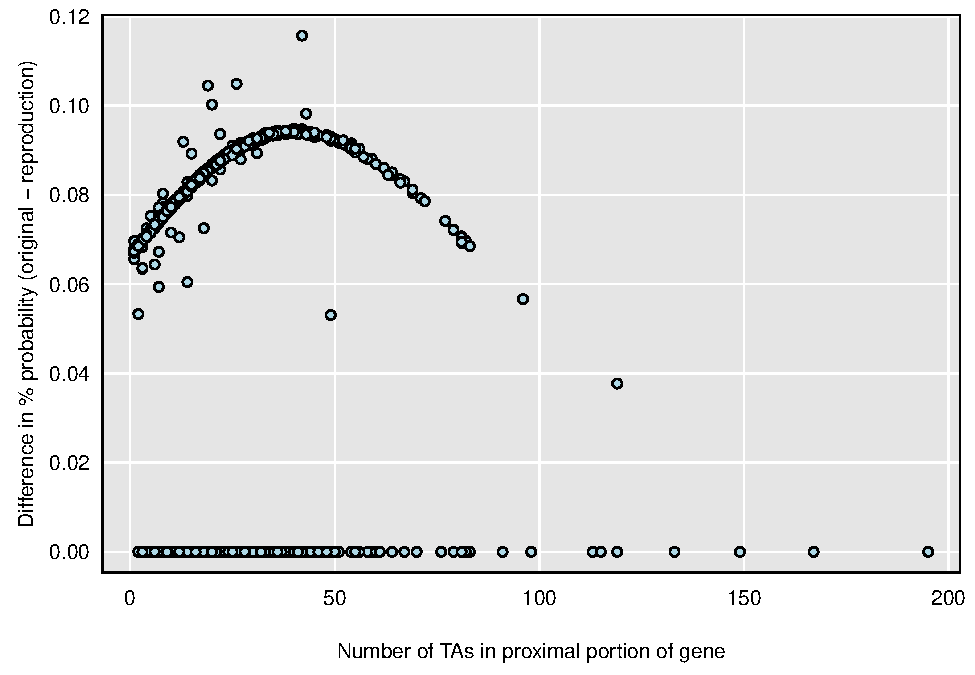
\includegraphics[width=0.7\textwidth]{../reproduction/Figs/fig2_diff.pdf}

\caption{Differences in estimated percent probability of being
essential, for the original results versus the reproduced values, for
each gene. That is, the difference in the y-axis values between the
left and right panels in Figure~\ref{fig:fig2} above,
$\times$100, \label{fig:fig2diff}}
\end{figure}


The genes with highest posterior probability of being essential are
shown in Table~\ref{tab:tab6}, a reproduction of Supplementary Table~6
from \citet{lamichhane2003}.
(Table~3 in \citet{lamichhane2003} showed just a subset of
these, omitting those indicated with an asterisk.) The original and
reproduced values, rounded to the nearest 1\%, are identical.

\begin{table}
\caption{Reproduction of Supplementary Table~6 from \citet{lamichhane2003},
\emph{M.\ tuberculosis\/} genes with high probabilities of being
essential. Genes indicated with * are the ones that were not also
included in Table 3 from \citet{lamichhane2003}.\label{tab:tab6}}

\centering
% latex table generated in R 3.6.1 by xtable 1.8-4 package
% Fri Feb 14 19:18:38 2020
\begin{tabular}{ccccc}
  \hline
  & & & \multicolumn{2}{c}{Probability (\%)}\\ MT \# & Rv \# & Gene description & original & reproduction\\ \hline
0418 & 0405 & Polyketide synthase (pks6)*  & 93 & 93 \\ 
  1218 & 1181 & Polyketide synthase  (pks4)*  & 88 & 88 \\ 
  3003 & 2933 & Phenolphthiocerol synthesis*  & 84 & 84 \\ 
  0417 & 0404 & Acyl-CoA synthase (fadD30) & 83 & 83 \\ 
  1701 & 1661 & Polyketide synthase (pks7)*  & 83 & 83 \\ 
  2062 & 2006 & Trehalose-6-phosphatase & 83 & 83 \\ 
  3285 & 3193c & Probable integral membrane protein & 83 & 83 \\ 
  2448 & 2380c & Mycobactin/Exochelin synthesis*  & 83 & 83 \\ 
  2082 & 2024c & Conserved hypothetical protein & 82 & 82 \\ 
  3974 & 3859c & Glutamate synthase (gltB) & 82 & 82 \\ 
  1587 & 1536 & Isoleucyl-tRNA synthase & 81 & 81 \\ 
  1198 & 1161 & Nitrate reductase[a]subunit (narG) & 79 & 79 \\ 
  0047 & 0041 & Leucyl-tRNA synthase (leuS) & 79 & 79 \\ 
  3002 & 2932 & Phenolphthiocerol synthesis*  & 78 & 78 \\ 
  2600 & 2524c & Fatty acid synthase (fasI) & 78 & 78 \\ 
  0070 & 0064 & Probable membrane protein & 77 & 77 \\ 
  1678 & 1640c & C-term Lysyl-tRNA synthase (lysX) & 76 & 76 \\ 
  1702 & 1662 & Polyketide synthase (pks8)*  & 76 & 76 \\ 
  2551 & 2476c & Conserved hypothetical protein & 75 & 75 \\ 
  1796 & 1753c & PPE-family protein & 75 & 75 \\ 
  0116 & 0107c & Probable Mg transport ATPase & 75 & 75 \\ 
  3045 & 2967c & Pyruvate carboxylase & 75 & 75 \\ 
   \hline
\end{tabular}

\end{table}

Finally, Table~\ref{tab:tab4} is a reproduction of Table~4
from \citet{lamichhane2003}, concerning an investigation of gene families,
to see whether particular families appeared to have an unusually high
or low proportion of essential genes. A few small differences between
the original and the reproduced values are highlighted in red: the
enrichment probability for three families changed by $\pm$1\%,
and the upper limit of the 95\% credible interval for the percent
essential genes in two families changed a bit. These changes can be
ascribed to MCMC sampling error.

\begin{table}
\caption{Reproduction of Table 4 from \citet{lamichhane2003},
\emph{M.\ tuberculosis\/} gene families enriched or deficient in
essential genes. Five changes are indicated in red.\label{tab:tab4}}

\centering
\small
% latex table generated in R 3.6.2 by xtable 1.8-4 package
% Sun Feb 23 09:00:36 2020
\begin{tabular}{lccc@{ (}r@{--}lc@{ (}r@{--}l}
  \hline
  & \multicolumn{2}{c}{Probability enriched (\%)} & \multicolumn{6}{c}{Est. \% essential}\\ Functional group & original & reproduction & \multicolumn{3}{c}{original} & \multicolumn{3}{c}{reproduction}\\ \hline
Aminoacyl tRNA synthases... & 97 & 97 & 54 & 32 & 76) & 54 & 32 & \textbf{\color{red} 72}) \\ 
  PE family: PGRS subfamily & 94 & \textbf{\color{red} 93} & 45 & 30 & 60) & 45 & 30 & 60) \\ 
  Purine ribonucleotide biosynthesis & 82 & 82 & 46 & 21 & 68) & 46 & 21 & 68) \\ 
  Polyketide and nonribosomal... & 80 & \textbf{\color{red} 81} & 40 & 28 & 52) & 40 & 28 & 52) \\ 
  Synthesis of fatty and mycolic acids & 78 & 78 & 42 & 23 & 62) & 42 & 23 & 62) \\ 
  Ser/Thr protein kinases and... & 75 & 75 & 43 & 21 & 64) & 43 & 21 & 64) \\ 
  Biosynthesis of molybdopterin & 75 & 75 & 42 & 20 & 65) & 42 & 20 & 65) \\ 
  Unknown proteins & 4 & 4 & 32 & 25 & 39) & 32 & 25 & 39) \\ 
  Metabolism of sulphur & 4 & \textbf{\color{red} 5} & 20 & 7 & 40) & 20 & 7 & 40) \\ 
  PPE family & 4 & 4 & 27 & 17 & 36) & 27 & 17 & \textbf{\color{red} 38}) \\ 
  Conserved membrane proteins & 0 & 0 & 10 & 0 & 24) & 10 & 0 & 24) \\ 
   \hline
\end{tabular}

\end{table}





\section{Lessons}


My efforts to reproduce the analyses for \citet{lamichhane2003} were
largely successful, but the process would have been considerably
easier had I put a bit more effort into file organization and
documentation. This work may serve as a useful case study to
illustrate the need for \emph{Good enough practices in scientific
computing} \citep{wilson2017}.

The two most important lessons from this effort are to document your
work, and to put all relevant scripts into a common project directory.
The quirks of my file organization would have been more easily
overcome if I had included a single {\tt ReadMe} file that explained
things. And it was only by luck that I identified the code for one of
the figures in a separate directory with slides for a talk.

The project organization would have been simpler had I
adopted a formal version control system like
\href{https://git-scm.com}{git}. This would have allowed me to avoid
the copy-and-mutate approach that led to the {\tt Sept02} and {\tt
Nov02} subdirectories. I should have combined the multiple mutated
versions of scripts into unified versions that provide the
comprehensive set of analysis results for the paper and relied on the
version control system to document the history of changes. A unified
analysis script, or even better a reproducible document such as in R
Markdown \citep{rmarkdown-book,rmarkdown-pkg}, would have made the
workflow more transparent.

For analyses that rely on random number generation, storing the seeds
could enable exact reproduction of the results. I should have also
saved intermediate results to files and loaded them at the top of
scripts that depended on them.

Finally, I should have documented the provenance of the primary data
files, such as that for the \emph{M.\ tuberculosis\/} genome.
